\documentclass{article}

% ============================================================
% INFR11269 Machine Learning Systems — Coursework Report
% Academic year 2026/27
%
% This coursework uses the official ICLR 2027 LaTeX style.
%
% IMPORTANT FORMAT RULES
% - Do not edit iclr2027_conference.sty.
% - Do not change page geometry, text width/height, base font size,
%   or line spacing.
% - Do not enable \iclrfinalcopy.
% - Normal content packages are fine if they do not alter the report format.
%
% Main-body page limit: six pages.
% References and Appendix do NOT count toward the main-body page limit.
% Reviewers are not obliged to read Appendix at all. Please put your main content
% in the main body.
%
% AI policy:
% Academic integrity is an underlying principle of research and academic practice.
% All submitted work is expected to be your own, including any material you have
% generated yourself with the assistance of AI tools such as ELM, ChatGPT,
% Bing Chat, Claude, Google Gemini, or any other automated assistance.
% For all such material you must make prominent explicit acknowledgement and
% explain clearly what you have done in the AI declaration section.
% This includes using AI to directly generate text, code, figures or similar
% or to complete other tasks. In all cases, you remain entirely responsible
% for the material you produce.
% ============================================================

\usepackage{iclr2027_conference,times}

\usepackage{hyperref}
\usepackage{url}
\usepackage{booktabs}
\usepackage{graphicx}
\usepackage{amsmath}
\usepackage{amssymb}
\usepackage{pgfplots}
\pgfplotsset{compat=1.18}
\usetikzlibrary{positioning,arrows.meta}

% The official ICLR archive includes math_commands.tex. It is optional:
%%%%% NEW MATH DEFINITIONS %%%%%

\usepackage{amsmath,amsfonts,bm}

% Mark sections of captions for referring to divisions of figures
\newcommand{\figleft}{{\em (Left)}}
\newcommand{\figcenter}{{\em (Center)}}
\newcommand{\figright}{{\em (Right)}}
\newcommand{\figtop}{{\em (Top)}}
\newcommand{\figbottom}{{\em (Bottom)}}
\newcommand{\captiona}{{\em (a)}}
\newcommand{\captionb}{{\em (b)}}
\newcommand{\captionc}{{\em (c)}}
\newcommand{\captiond}{{\em (d)}}

% Highlight a newly defined term
\newcommand{\newterm}[1]{{\bf #1}}


% Figure reference, lower-case.
\def\figref#1{figure~\ref{#1}}
% Figure reference, capital. For start of sentence
\def\Figref#1{Figure~\ref{#1}}
\def\twofigref#1#2{figures \ref{#1} and \ref{#2}}
\def\quadfigref#1#2#3#4{figures \ref{#1}, \ref{#2}, \ref{#3} and \ref{#4}}
% Section reference, lower-case.
\def\secref#1{section~\ref{#1}}
% Section reference, capital.
\def\Secref#1{Section~\ref{#1}}
% Reference to two sections.
\def\twosecrefs#1#2{sections \ref{#1} and \ref{#2}}
% Reference to three sections.
\def\secrefs#1#2#3{sections \ref{#1}, \ref{#2} and \ref{#3}}
% Reference to an equation, lower-case.
\def\eqref#1{equation~\ref{#1}}
% Reference to an equation, upper case
\def\Eqref#1{Equation~\ref{#1}}
% A raw reference to an equation---avoid using if possible
\def\plaineqref#1{\ref{#1}}
% Reference to a chapter, lower-case.
\def\chapref#1{chapter~\ref{#1}}
% Reference to an equation, upper case.
\def\Chapref#1{Chapter~\ref{#1}}
% Reference to a range of chapters
\def\rangechapref#1#2{chapters\ref{#1}--\ref{#2}}
% Reference to an algorithm, lower-case.
\def\algref#1{algorithm~\ref{#1}}
% Reference to an algorithm, upper case.
\def\Algref#1{Algorithm~\ref{#1}}
\def\twoalgref#1#2{algorithms \ref{#1} and \ref{#2}}
\def\Twoalgref#1#2{Algorithms \ref{#1} and \ref{#2}}
% Reference to a part, lower case
\def\partref#1{part~\ref{#1}}
% Reference to a part, upper case
\def\Partref#1{Part~\ref{#1}}
\def\twopartref#1#2{parts \ref{#1} and \ref{#2}}

\def\ceil#1{\lceil #1 \rceil}
\def\floor#1{\lfloor #1 \rfloor}
\def\1{\bm{1}}
\newcommand{\train}{\mathcal{D}}
\newcommand{\valid}{\mathcal{D_{\mathrm{valid}}}}
\newcommand{\test}{\mathcal{D_{\mathrm{test}}}}

\def\eps{{\epsilon}}


% Random variables
\def\reta{{\textnormal{$\eta$}}}
\def\ra{{\textnormal{a}}}
\def\rb{{\textnormal{b}}}
\def\rc{{\textnormal{c}}}
\def\rd{{\textnormal{d}}}
\def\re{{\textnormal{e}}}
\def\rf{{\textnormal{f}}}
\def\rg{{\textnormal{g}}}
\def\rh{{\textnormal{h}}}
\def\ri{{\textnormal{i}}}
\def\rj{{\textnormal{j}}}
\def\rk{{\textnormal{k}}}
\def\rl{{\textnormal{l}}}
% rm is already a command, just don't name any random variables m
\def\rn{{\textnormal{n}}}
\def\ro{{\textnormal{o}}}
\def\rp{{\textnormal{p}}}
\def\rq{{\textnormal{q}}}
\def\rr{{\textnormal{r}}}
\def\rs{{\textnormal{s}}}
\def\rt{{\textnormal{t}}}
\def\ru{{\textnormal{u}}}
\def\rv{{\textnormal{v}}}
\def\rw{{\textnormal{w}}}
\def\rx{{\textnormal{x}}}
\def\ry{{\textnormal{y}}}
\def\rz{{\textnormal{z}}}

% Random vectors
\def\rvepsilon{{\mathbf{\epsilon}}}
\def\rvtheta{{\mathbf{\theta}}}
\def\rva{{\mathbf{a}}}
\def\rvb{{\mathbf{b}}}
\def\rvc{{\mathbf{c}}}
\def\rvd{{\mathbf{d}}}
\def\rve{{\mathbf{e}}}
\def\rvf{{\mathbf{f}}}
\def\rvg{{\mathbf{g}}}
\def\rvh{{\mathbf{h}}}
\def\rvu{{\mathbf{i}}}
\def\rvj{{\mathbf{j}}}
\def\rvk{{\mathbf{k}}}
\def\rvl{{\mathbf{l}}}
\def\rvm{{\mathbf{m}}}
\def\rvn{{\mathbf{n}}}
\def\rvo{{\mathbf{o}}}
\def\rvp{{\mathbf{p}}}
\def\rvq{{\mathbf{q}}}
\def\rvr{{\mathbf{r}}}
\def\rvs{{\mathbf{s}}}
\def\rvt{{\mathbf{t}}}
\def\rvu{{\mathbf{u}}}
\def\rvv{{\mathbf{v}}}
\def\rvw{{\mathbf{w}}}
\def\rvx{{\mathbf{x}}}
\def\rvy{{\mathbf{y}}}
\def\rvz{{\mathbf{z}}}

% Elements of random vectors
\def\erva{{\textnormal{a}}}
\def\ervb{{\textnormal{b}}}
\def\ervc{{\textnormal{c}}}
\def\ervd{{\textnormal{d}}}
\def\erve{{\textnormal{e}}}
\def\ervf{{\textnormal{f}}}
\def\ervg{{\textnormal{g}}}
\def\ervh{{\textnormal{h}}}
\def\ervi{{\textnormal{i}}}
\def\ervj{{\textnormal{j}}}
\def\ervk{{\textnormal{k}}}
\def\ervl{{\textnormal{l}}}
\def\ervm{{\textnormal{m}}}
\def\ervn{{\textnormal{n}}}
\def\ervo{{\textnormal{o}}}
\def\ervp{{\textnormal{p}}}
\def\ervq{{\textnormal{q}}}
\def\ervr{{\textnormal{r}}}
\def\ervs{{\textnormal{s}}}
\def\ervt{{\textnormal{t}}}
\def\ervu{{\textnormal{u}}}
\def\ervv{{\textnormal{v}}}
\def\ervw{{\textnormal{w}}}
\def\ervx{{\textnormal{x}}}
\def\ervy{{\textnormal{y}}}
\def\ervz{{\textnormal{z}}}

% Random matrices
\def\rmA{{\mathbf{A}}}
\def\rmB{{\mathbf{B}}}
\def\rmC{{\mathbf{C}}}
\def\rmD{{\mathbf{D}}}
\def\rmE{{\mathbf{E}}}
\def\rmF{{\mathbf{F}}}
\def\rmG{{\mathbf{G}}}
\def\rmH{{\mathbf{H}}}
\def\rmI{{\mathbf{I}}}
\def\rmJ{{\mathbf{J}}}
\def\rmK{{\mathbf{K}}}
\def\rmL{{\mathbf{L}}}
\def\rmM{{\mathbf{M}}}
\def\rmN{{\mathbf{N}}}
\def\rmO{{\mathbf{O}}}
\def\rmP{{\mathbf{P}}}
\def\rmQ{{\mathbf{Q}}}
\def\rmR{{\mathbf{R}}}
\def\rmS{{\mathbf{S}}}
\def\rmT{{\mathbf{T}}}
\def\rmU{{\mathbf{U}}}
\def\rmV{{\mathbf{V}}}
\def\rmW{{\mathbf{W}}}
\def\rmX{{\mathbf{X}}}
\def\rmY{{\mathbf{Y}}}
\def\rmZ{{\mathbf{Z}}}

% Elements of random matrices
\def\ermA{{\textnormal{A}}}
\def\ermB{{\textnormal{B}}}
\def\ermC{{\textnormal{C}}}
\def\ermD{{\textnormal{D}}}
\def\ermE{{\textnormal{E}}}
\def\ermF{{\textnormal{F}}}
\def\ermG{{\textnormal{G}}}
\def\ermH{{\textnormal{H}}}
\def\ermI{{\textnormal{I}}}
\def\ermJ{{\textnormal{J}}}
\def\ermK{{\textnormal{K}}}
\def\ermL{{\textnormal{L}}}
\def\ermM{{\textnormal{M}}}
\def\ermN{{\textnormal{N}}}
\def\ermO{{\textnormal{O}}}
\def\ermP{{\textnormal{P}}}
\def\ermQ{{\textnormal{Q}}}
\def\ermR{{\textnormal{R}}}
\def\ermS{{\textnormal{S}}}
\def\ermT{{\textnormal{T}}}
\def\ermU{{\textnormal{U}}}
\def\ermV{{\textnormal{V}}}
\def\ermW{{\textnormal{W}}}
\def\ermX{{\textnormal{X}}}
\def\ermY{{\textnormal{Y}}}
\def\ermZ{{\textnormal{Z}}}

% Vectors
\def\vzero{{\bm{0}}}
\def\vone{{\bm{1}}}
\def\vmu{{\bm{\mu}}}
\def\vtheta{{\bm{\theta}}}
\def\va{{\bm{a}}}
\def\vb{{\bm{b}}}
\def\vc{{\bm{c}}}
\def\vd{{\bm{d}}}
\def\ve{{\bm{e}}}
\def\vf{{\bm{f}}}
\def\vg{{\bm{g}}}
\def\vh{{\bm{h}}}
\def\vi{{\bm{i}}}
\def\vj{{\bm{j}}}
\def\vk{{\bm{k}}}
\def\vl{{\bm{l}}}
\def\vm{{\bm{m}}}
\def\vn{{\bm{n}}}
\def\vo{{\bm{o}}}
\def\vp{{\bm{p}}}
\def\vq{{\bm{q}}}
\def\vr{{\bm{r}}}
\def\vs{{\bm{s}}}
\def\vt{{\bm{t}}}
\def\vu{{\bm{u}}}
\def\vv{{\bm{v}}}
\def\vw{{\bm{w}}}
\def\vx{{\bm{x}}}
\def\vy{{\bm{y}}}
\def\vz{{\bm{z}}}

% Elements of vectors
\def\evalpha{{\alpha}}
\def\evbeta{{\beta}}
\def\evepsilon{{\epsilon}}
\def\evlambda{{\lambda}}
\def\evomega{{\omega}}
\def\evmu{{\mu}}
\def\evpsi{{\psi}}
\def\evsigma{{\sigma}}
\def\evtheta{{\theta}}
\def\eva{{a}}
\def\evb{{b}}
\def\evc{{c}}
\def\evd{{d}}
\def\eve{{e}}
\def\evf{{f}}
\def\evg{{g}}
\def\evh{{h}}
\def\evi{{i}}
\def\evj{{j}}
\def\evk{{k}}
\def\evl{{l}}
\def\evm{{m}}
\def\evn{{n}}
\def\evo{{o}}
\def\evp{{p}}
\def\evq{{q}}
\def\evr{{r}}
\def\evs{{s}}
\def\evt{{t}}
\def\evu{{u}}
\def\evv{{v}}
\def\evw{{w}}
\def\evx{{x}}
\def\evy{{y}}
\def\evz{{z}}

% Matrix
\def\mA{{\bm{A}}}
\def\mB{{\bm{B}}}
\def\mC{{\bm{C}}}
\def\mD{{\bm{D}}}
\def\mE{{\bm{E}}}
\def\mF{{\bm{F}}}
\def\mG{{\bm{G}}}
\def\mH{{\bm{H}}}
\def\mI{{\bm{I}}}
\def\mJ{{\bm{J}}}
\def\mK{{\bm{K}}}
\def\mL{{\bm{L}}}
\def\mM{{\bm{M}}}
\def\mN{{\bm{N}}}
\def\mO{{\bm{O}}}
\def\mP{{\bm{P}}}
\def\mQ{{\bm{Q}}}
\def\mR{{\bm{R}}}
\def\mS{{\bm{S}}}
\def\mT{{\bm{T}}}
\def\mU{{\bm{U}}}
\def\mV{{\bm{V}}}
\def\mW{{\bm{W}}}
\def\mX{{\bm{X}}}
\def\mY{{\bm{Y}}}
\def\mZ{{\bm{Z}}}
\def\mBeta{{\bm{\beta}}}
\def\mPhi{{\bm{\Phi}}}
\def\mLambda{{\bm{\Lambda}}}
\def\mSigma{{\bm{\Sigma}}}

% Tensor
\DeclareMathAlphabet{\mathsfit}{\encodingdefault}{\sfdefault}{m}{sl}
\SetMathAlphabet{\mathsfit}{bold}{\encodingdefault}{\sfdefault}{bx}{n}
\newcommand{\tens}[1]{\bm{\mathsfit{#1}}}
\def\tA{{\tens{A}}}
\def\tB{{\tens{B}}}
\def\tC{{\tens{C}}}
\def\tD{{\tens{D}}}
\def\tE{{\tens{E}}}
\def\tF{{\tens{F}}}
\def\tG{{\tens{G}}}
\def\tH{{\tens{H}}}
\def\tI{{\tens{I}}}
\def\tJ{{\tens{J}}}
\def\tK{{\tens{K}}}
\def\tL{{\tens{L}}}
\def\tM{{\tens{M}}}
\def\tN{{\tens{N}}}
\def\tO{{\tens{O}}}
\def\tP{{\tens{P}}}
\def\tQ{{\tens{Q}}}
\def\tR{{\tens{R}}}
\def\tS{{\tens{S}}}
\def\tT{{\tens{T}}}
\def\tU{{\tens{U}}}
\def\tV{{\tens{V}}}
\def\tW{{\tens{W}}}
\def\tX{{\tens{X}}}
\def\tY{{\tens{Y}}}
\def\tZ{{\tens{Z}}}


% Graph
\def\gA{{\mathcal{A}}}
\def\gB{{\mathcal{B}}}
\def\gC{{\mathcal{C}}}
\def\gD{{\mathcal{D}}}
\def\gE{{\mathcal{E}}}
\def\gF{{\mathcal{F}}}
\def\gG{{\mathcal{G}}}
\def\gH{{\mathcal{H}}}
\def\gI{{\mathcal{I}}}
\def\gJ{{\mathcal{J}}}
\def\gK{{\mathcal{K}}}
\def\gL{{\mathcal{L}}}
\def\gM{{\mathcal{M}}}
\def\gN{{\mathcal{N}}}
\def\gO{{\mathcal{O}}}
\def\gP{{\mathcal{P}}}
\def\gQ{{\mathcal{Q}}}
\def\gR{{\mathcal{R}}}
\def\gS{{\mathcal{S}}}
\def\gT{{\mathcal{T}}}
\def\gU{{\mathcal{U}}}
\def\gV{{\mathcal{V}}}
\def\gW{{\mathcal{W}}}
\def\gX{{\mathcal{X}}}
\def\gY{{\mathcal{Y}}}
\def\gZ{{\mathcal{Z}}}

% Sets
\def\sA{{\mathbb{A}}}
\def\sB{{\mathbb{B}}}
\def\sC{{\mathbb{C}}}
\def\sD{{\mathbb{D}}}
% Don't use a set called E, because this would be the same as our symbol
% for expectation.
\def\sF{{\mathbb{F}}}
\def\sG{{\mathbb{G}}}
\def\sH{{\mathbb{H}}}
\def\sI{{\mathbb{I}}}
\def\sJ{{\mathbb{J}}}
\def\sK{{\mathbb{K}}}
\def\sL{{\mathbb{L}}}
\def\sM{{\mathbb{M}}}
\def\sN{{\mathbb{N}}}
\def\sO{{\mathbb{O}}}
\def\sP{{\mathbb{P}}}
\def\sQ{{\mathbb{Q}}}
\def\sR{{\mathbb{R}}}
\def\sS{{\mathbb{S}}}
\def\sT{{\mathbb{T}}}
\def\sU{{\mathbb{U}}}
\def\sV{{\mathbb{V}}}
\def\sW{{\mathbb{W}}}
\def\sX{{\mathbb{X}}}
\def\sY{{\mathbb{Y}}}
\def\sZ{{\mathbb{Z}}}

% Entries of a matrix
\def\emLambda{{\Lambda}}
\def\emA{{A}}
\def\emB{{B}}
\def\emC{{C}}
\def\emD{{D}}
\def\emE{{E}}
\def\emF{{F}}
\def\emG{{G}}
\def\emH{{H}}
\def\emI{{I}}
\def\emJ{{J}}
\def\emK{{K}}
\def\emL{{L}}
\def\emM{{M}}
\def\emN{{N}}
\def\emO{{O}}
\def\emP{{P}}
\def\emQ{{Q}}
\def\emR{{R}}
\def\emS{{S}}
\def\emT{{T}}
\def\emU{{U}}
\def\emV{{V}}
\def\emW{{W}}
\def\emX{{X}}
\def\emY{{Y}}
\def\emZ{{Z}}
\def\emSigma{{\Sigma}}

% entries of a tensor
% Same font as tensor, without \bm wrapper
\newcommand{\etens}[1]{\mathsfit{#1}}
\def\etLambda{{\etens{\Lambda}}}
\def\etA{{\etens{A}}}
\def\etB{{\etens{B}}}
\def\etC{{\etens{C}}}
\def\etD{{\etens{D}}}
\def\etE{{\etens{E}}}
\def\etF{{\etens{F}}}
\def\etG{{\etens{G}}}
\def\etH{{\etens{H}}}
\def\etI{{\etens{I}}}
\def\etJ{{\etens{J}}}
\def\etK{{\etens{K}}}
\def\etL{{\etens{L}}}
\def\etM{{\etens{M}}}
\def\etN{{\etens{N}}}
\def\etO{{\etens{O}}}
\def\etP{{\etens{P}}}
\def\etQ{{\etens{Q}}}
\def\etR{{\etens{R}}}
\def\etS{{\etens{S}}}
\def\etT{{\etens{T}}}
\def\etU{{\etens{U}}}
\def\etV{{\etens{V}}}
\def\etW{{\etens{W}}}
\def\etX{{\etens{X}}}
\def\etY{{\etens{Y}}}
\def\etZ{{\etens{Z}}}

% The true underlying data generating distribution
\newcommand{\pdata}{p_{\rm{data}}}
% The empirical distribution defined by the training set
\newcommand{\ptrain}{\hat{p}_{\rm{data}}}
\newcommand{\Ptrain}{\hat{P}_{\rm{data}}}
% The model distribution
\newcommand{\pmodel}{p_{\rm{model}}}
\newcommand{\Pmodel}{P_{\rm{model}}}
\newcommand{\ptildemodel}{\tilde{p}_{\rm{model}}}
% Stochastic autoencoder distributions
\newcommand{\pencode}{p_{\rm{encoder}}}
\newcommand{\pdecode}{p_{\rm{decoder}}}
\newcommand{\precons}{p_{\rm{reconstruct}}}

\newcommand{\laplace}{\mathrm{Laplace}} % Laplace distribution

\newcommand{\E}{\mathbb{E}}
\newcommand{\Ls}{\mathcal{L}}
\newcommand{\R}{\mathbb{R}}
\newcommand{\emp}{\tilde{p}}
\newcommand{\lr}{\alpha}
\newcommand{\reg}{\lambda}
\newcommand{\rect}{\mathrm{rectifier}}
\newcommand{\softmax}{\mathrm{softmax}}
\newcommand{\sigmoid}{\sigma}
\newcommand{\softplus}{\zeta}
\newcommand{\KL}{D_{\mathrm{KL}}}
\newcommand{\Var}{\mathrm{Var}}
\newcommand{\standarderror}{\mathrm{SE}}
\newcommand{\Cov}{\mathrm{Cov}}
% Wolfram Mathworld says $L^2$ is for function spaces and $\ell^2$ is for vectors
% But then they seem to use $L^2$ for vectors throughout the site, and so does
% wikipedia.
\newcommand{\normlzero}{L^0}
\newcommand{\normlone}{L^1}
\newcommand{\normltwo}{L^2}
\newcommand{\normlp}{L^p}
\newcommand{\normmax}{L^\infty}

\newcommand{\parents}{Pa} % See usage in notation.tex. Chosen to match Daphne's book.

\DeclareMathOperator*{\argmax}{arg\,max}
\DeclareMathOperator*{\argmin}{arg\,min}

\DeclareMathOperator{\sign}{sign}
\DeclareMathOperator{\Tr}{Tr}
\let\ab\allowbreak


\title{Spoken-question RAG on our own CUDA kernels: does cross-encoder reranking pay for itself?}

% Keep this line unchanged.
\author{Anonymous coursework submission}

% Keep this COMMENTED OUT.
% Review mode is part of the coursework format and is checked automatically.
% \iclrfinalcopy

\begin{document}

\maketitle

% Course-specific template fingerprint. Keep this line unchanged.
\lhead{Under review as a report for UoE 26/27 Sem1 INFR11269: Machine Learning Systems}

% Keep this COMMENTED OUT.
% \begin{abstract}
% \end{abstract}

\section{Introduction}
\label{sec:introduction}

Our system answers spoken questions about 24{,}000 posts from a personal-finance forum. A speech recogniser (ASR) turns the audio into text, a small encoder (\texttt{enc\_a}) turns the text into a vector, exact search finds the 5 closest posts, and a language model on the University ELM service writes an answer from them~\citep{lewis2020rag}. We wrote the CUDA kernels that the ASR model runs on, and we added a reranking stage to the retrieval path and measured what it changes.

\texttt{enc\_a} scores the question and each record separately. A cross-encoder reads the question and one record together, which usually ranks better but costs one transformer pass per record~\citep{nogueira2019passage}. There is room for a better order. On the practice split, 77\% of the relevant records are in \texttt{enc\_a}'s top 100, but only 42\% reach the top 5 that the language model sees, and answers to questions with no relevant record in the top 5 score 0.14 on average, against 0.47 for the rest (Section~\ref{sec:why}). We ask:

\begin{quote}
\emph{Does reranking \texttt{enc\_a}'s top-$N$ candidates with an off-the-shelf cross-encoder put more relevant records in the top 5 and give better answers, and what does it cost in latency, GPU memory and prompt size?}
\end{quote}

Our kernels pass all 33 test cases and transcribe the test clip exactly, but the model runs 3.0$\times$ slower than with PyTorch, mostly because of our matrix multiply (Section~\ref{sec:asr-results}); the task-guide answers are in Section~\ref{sec:guide}. Reranking did not clearly help. On the 125-question dev split the better reranker raised the mean judge score by 0.035 (95\% CI $-0.021$ to $+0.089$), while adding 61--111\,ms per question, up to 1.6\,GB of GPU memory and 8--21\% longer prompts. The rerankers often pushed a correct first result down; where they did raise Recall@5, the answers improved.

\section{The system and our changes}
\label{sec:approach}

\begin{figure}[h]
\centering
\resizebox{\linewidth}{!}{%
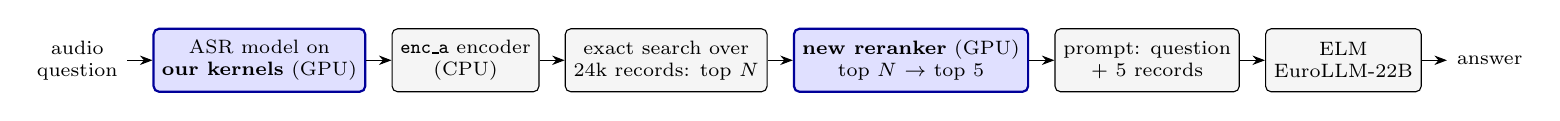
\begin{tikzpicture}[font=\scriptsize, node distance=0.32cm,
  box/.style={draw, rounded corners=2pt, align=center, minimum height=0.8cm, inner sep=3pt},
  sup/.style={box, fill=gray!8},
  ours/.style={box, fill=blue!12, draw=blue!60!black, thick},
  arr/.style={-{Stealth[length=1.6mm]}}]
\node[align=center] (audio) {audio\\question};
\node[ours, right=of audio] (asr) {ASR model on\\\textbf{our kernels} (GPU)};
\node[sup, right=of asr] (enc) {\texttt{enc\_a} encoder\\(CPU)};
\node[sup, right=of enc] (ret) {exact search over\\24k records: top $N$};
\node[ours, right=of ret] (rr) {\textbf{new reranker} (GPU)\\top $N$ $\rightarrow$ top 5};
\node[sup, right=of rr] (ctx) {prompt: question\\+ 5 records};
\node[sup, right=of ctx] (llm) {ELM\\EuroLLM-22B};
\node[right=of llm] (ans) {answer};
\draw[arr] (audio) -- (asr);
\draw[arr] (asr) -- (enc);
\draw[arr] (enc) -- (ret);
\draw[arr] (ret) -- (rr);
\draw[arr] (rr) -- (ctx);
\draw[arr] (ctx) -- (llm);
\draw[arr] (llm) -- (ans);
\end{tikzpicture}}
\caption{The pipeline. Blue: our work (the kernels in the five task files; the reranking stage with its scripts, tests, transcript reuse and judge-output fallback). Grey: supplied, including the ASR model code, \texttt{enc\_a}, exact search, prompt builder, ELM generator, and the LLM judge used only for evaluation. The baseline has no reranker.}
\label{fig:pipeline}
\end{figure}

\subsection{ASR kernels}
\label{sec:kernels}

The supplied GLM-ASR-Nano model has about 2.3B float32 parameters (9\,GB). Audio is padded to 30\,s, so the encoder always runs 32 layers over 1500 positions; the 28-layer decoder writes tokens greedily and without a KV cache, so each step recomputes all positions.

\emph{RoPE (Task 1)} rotates pairs of numbers in each query and key vector by an angle that depends on the position~\citep{su2024roformer}. One thread handles one pair, and one launch covers both $q$ and $k$, halving the fixed launch cost over 396 calls. With almost no arithmetic, its speed depends on coalesced access: neighbouring threads touch neighbouring addresses.

\emph{Reductions (Task 2).} A warp sums its 32 values in five shuffle steps, without shared memory; a block of 256 threads then combines its 8 warp results through a small shared array. Empty slots in the block maximum hold $-\infty$, not 0, so a row of negative numbers still gives the right answer. Softmax keeps a running pair (maximum, sum of exponentials) and merges pairs as it goes~\citep{milakov2018online}, so it reads the row twice instead of three times. Merging two empty pairs is handled separately, because $-\infty-(-\infty)$ is NaN.

\emph{Tiled GEMM (Task 3)} computes $y=\mathrm{act}(xW^\top+b)$ with $W$ stored as $[N,K]$. Each $16\times16$ thread block copies $16\times16$ tiles of $x$ and $W$ into shared memory, where each value is then used 16 times. We load the $W$ tile with $k$ following \texttt{threadIdx.x}, so the reads stay coalesced although $W$ is transposed, and we pad it to $16\times17$ to avoid bank conflicts. Bias and GELU are applied before the store, so the $1500\times5120$ output of \texttt{fc1} is not written out and read back by a separate kernel. No thread returns early, since all threads must reach both barriers.

\emph{Attention (Task 4)} never stores the score matrix, as in FlashAttention~\citep{dao2022flashattention}. A block of 4 warps handles 4 queries, which share each copy of 32 keys and 32 values in shared memory. Each warp keeps a running maximum, sum and weighted sum of values, and rescales them when a larger score appears. The kernel supports grouped-query attention~\citep{ainslie2023gqa} and the causal mask.

\subsection{Reranking stage}
\label{sec:rerank}

We split the pipeline after ASR: a new function, \texttt{answer\_transcript}, runs everything from the transcript onward. With a reranker set, it asks exact search for $N$ candidates instead of 5, scores the $N$ (question, record) pairs with a cross-encoder on the GPU, sorts them by score and keeps the top 5. The sort is stable, so ties keep \texttt{enc\_a}'s order. Without a reranker the original code path runs, and a unit test checks that it returns the same records. The prompt, $k{=}5$, the encoder and the language model do not change, so the choice and order of the 5 records is the only difference between conditions.

We chose reranking over three other options. A larger $k$ also brings in more relevant records, but it makes every prompt longer. An approximate index~\citep{johnson2021faiss,malkov2020hnsw} would speed up a search that already takes only 5\,ms. Mixing dense and reranker scores, or fine-tuning a reranker, needs tuning data, so we measured the plain reranker first. We compare two public models: \texttt{ms-marco-MiniLM-L-6-v2} (22M parameters, trained on MS MARCO web search~\citep{nguyen2016msmarco,wang2020minilm}) and \texttt{bge-reranker-base} (278M parameters, general training data~\citep{xiao2024cpack}). Both run through \texttt{sentence-transformers}~\citep{reimers2019sbert} with batches of 32 and at most 512 tokens per pair; longer pairs are cut at the end. We try $N \in \{10, 20, 50, 100\}$.

Two smaller changes support the experiment. Answer generation can now reuse cached ASR transcripts, so all conditions answer the same text. And the supplied judge crashed when the judge model returned slightly malformed JSON, which it does repeatably at temperature 0; our fallback reads the three scores with a regular expression and marks the row (20 of 350 practice and 9 of 375 dev judgements).

\section{How we evaluated}
\label{sec:methodology}

\textbf{Setup.} All GPU numbers come from one NVIDIA GeForce RTX 2080 Ti (68 SMs, 11\,GB, 616\,GB/s peak bandwidth). The kernels are built with CUDA 12.8 (\texttt{-O3}, \texttt{sm\_75}); the ASR environment uses PyTorch 2.10, and the RAG environment PyTorch 2.15 with Python 3.11. For HW1, \texttt{make test} checks each kernel against a CPU version and prints its speed; \texttt{run.sh} times three transcriptions of the 3.5\,s test clip after a warm-up, without model loading, and \texttt{--profile} gives GPU time per operation. All HW1 numbers come from one session on one node (Appendix~\ref{app:hw1}).

\textbf{RAG protocol.} We used the 350 practice questions to develop and to choose $N$ for each reranker, and report final numbers on the 125 dev questions. ASR ran once per split and the transcripts were cached, so every condition reads identical text (we checked all 125 dev transcripts). They come from the ASR adapter's default backend, our kernels (the median ASR time of 4.3\,s per question matches our kernels, not PyTorch, which is 3$\times$ faster); the comparisons do not depend on this. The generator is EuroLLM-22B-Instruct at temperature 0.1.

\textbf{Quality metrics.} Recall@5, the share of a question's relevant records that reach the top 5, is our main retrieval metric, because the model sees exactly 5 records. We also report MRR@10, NDCG@10 and an \emph{oracle} Recall@5, the best that any reordering of the top $N$ could reach. The supplied judge (EuroLLM-22B, temperature 0, one judgement per answer) scores correctness, grounding and completeness from 0 to 4 against the gold evidence; we use their sum divided by 12. The judge sees the ASR transcript as the question and is itself an LLM~\citep{zheng2023judge}, so we treat its scores as an aid and measure their noise (\S\ref{sec:answers}).

\textbf{Cost and timing boundaries.} \texttt{rerank\_ms} covers tokenising, the GPU forward pass and the sort, but not model loading, which we report separately. The latency benchmark makes no ELM calls: after 10 warm-up questions it reranks every dev question 5 times per $N$, and we report the median and 95th percentile of the 625 timings and the peak GPU memory. \texttt{generation\_ms} is one ELM call, including the network. In the dev runs \texttt{end\_to\_end\_ms} excludes ASR, because the transcripts are cached; the practice baseline run includes it. We report medians, as the first question of a run is slow and a few API calls took up to 185\,s.

\textbf{Statistics.} We compare conditions question by question, reporting the mean judge-score difference with a 95\% bootstrap interval (10{,}000 resamples)~\citep{efron1994bootstrap} and a sign-flip permutation $p$-value. The dev comparison used 375 generation and 375 judge calls.

\section{Results and analysis}
\label{sec:results}

\subsection{ASR kernels}
\label{sec:asr-results}

All 33 test cases pass, and on our kernels the model returns the reference transcription (100\% word accuracy). Table~\ref{tab:asr} compares the whole model with the supplied PyTorch version.

\begin{table}[t]
\caption{Whole model, ours vs the supplied PyTorch version (\texttt{run.sh --profile}, with and without \texttt{--cuda none}). Time per transcription: mean $\pm$ std of 3 runs. Operation rows: GPU time in one profiled transcription (profiling waits after each call); the other 5 operations take under 10\,ms in both.}
\label{tab:asr}
\centering\small
\begin{tabular}{lrrrr}
\toprule
 & \multicolumn{2}{c}{Ours} & \multicolumn{2}{c}{PyTorch} \\
\midrule
Time per transcription (ms) & \multicolumn{2}{r}{$3230.6 \pm 7.2$} & \multicolumn{2}{r}{$1065.0 \pm 0.2$} \\
Time per token (ms); peak GPU memory (GiB) & 248.5 & 8.56 & 81.9 & 8.88 \\
\midrule
linear (Task 3), 2757 calls: ms, share & 2832.1 & 83.3\% & 597.4 & 41.6\% \\
attention (Task 4), 396 calls & 547.3 & 16.1\% & 313.3 & 21.8\% \\
RMSNorm (Task 2), 741 calls & 6.7 & 0.2\% & 85.5 & 5.9\% \\
RoPE (Task 1), 396 calls & 3.0 & 0.1\% & 433.3 & 30.1\% \\
\bottomrule
\end{tabular}
\end{table}

The matrix multiply sets the speed. It takes 83\% of our GPU time, and our linear layers run 2235\,ms longer than PyTorch's, more than the whole 2166\,ms difference in wall time; our faster RoPE and RMSNorm win some of it back. On the large encoder shapes our kernel reaches 1.4--1.9\,TFLOP/s (encoder \texttt{q\_proj}: 1{,}939\,GFLOP/s, against 234 for the naive kernel and 13{,}195 for cuBLAS; all cases are in Appendix~\ref{app:hw1}). That is 6--8$\times$ the naive kernel but 7--10$\times$ below cuBLAS, which runs at about the card's nominal FP32 peak of 13.4\,TFLOP/s. Each multiply--add in our inner loop needs two shared-memory reads, so shared-memory traffic, not arithmetic, limits it. cuBLAS keeps a small block of inputs and outputs in each thread's registers, so one value read feeds several multiply--adds (register tiling~\citep{volkov2008benchmarking}), and it loads the next tile while computing the current one. For \texttt{lm\_head} ($M{=}1$) the work is reading a 485.5\,MB weight matrix; from the printed times we reach 250\,GB/s (41\% of peak) and cuBLAS 582\,GB/s. Each of our threads issues one 4-byte load per tile and then waits at a barrier, so few loads are in flight at once.

Our memory-bound kernels are fast when the input is large. On the encoder, RoPE reaches 490\,GB/s (80\% of peak) and LayerNorm 382\,GB/s (62\%). The decoder cases are too small to fill the GPU, and the 59{,}264-wide vocabulary softmax is a single row, so it runs as one block on one of the 68 SMs (3.6\,GB/s). These kernels also beat the PyTorch path by far (RoPE 3.0 vs 433.3\,ms, RMSNorm 6.7 vs 85.5\,ms): \texttt{ops.py} builds them from separate tensor operations (about two dozen for RoPE, six for RMSNorm), each with its own launch and pass over memory, while ours are one launch each.

\subsection{Answers to the task-guide questions}
\label{sec:guide}

We answer one question from each guide, using the \texttt{make test} run in Appendix~\ref{app:hw1}.

\textbf{Task 1, Question 1.} \emph{``For the audio encoder case, how many bytes does the kernel read and write in total? Which fraction of your GPU's peak bandwidth did you reach?''}
The encoder case has 60{,}000 rows (1500 positions $\times$ 40 heads) of 64 numbers, and RoPE rotates the first 32 of each. Each of those floats is read and written once: $60{,}000 \times 32 \times 4\,\text{B} \times 2 = 15.36$\,MB. At 0.031\,ms the test reports 490\,GB/s, which is 80\% of the 616\,GB/s peak. Accesses are coalesced: each row's rotated half is one aligned 128-byte segment. The tiny test cases take about 4\,\textmu s however small they are, so a few microseconds of every call are fixed launch and synchronisation cost. Without it the rate would be close to 90\% of peak, about what a plain copy reaches.

\textbf{Task 2, Question 4.} \emph{``Describe, as a sequence of events between two warps, what can go wrong in LayerNorm without the final \texttt{\_\_syncthreads()} in \texttt{block\_reduce\_sum}.''}
\texttt{block\_reduce\_sum} keeps the warp sums in one static shared array, \texttt{partial[32]}, and LayerNorm calls it twice: for the mean, then for the variance. In the last step every warp reads all slots. Without the final barrier: (1) warps 0 and 1 write their sums $S_0$ and $S_1$ and pass the first barrier; (2) warp 0 reads $S_0+S_1$, gets the right mean and moves on, while warp 1 is paused before its read; (3) warp 0 computes its part of the variance, $Q_0$, and writes it into \texttt{partial[0]} in the second call; (4) warp 1 reads $Q_0+S_1$ and gets a wrong mean. The row then has two different means and a wrong variance, so every output in it is silently wrong. Without the barrier \texttt{make test2} still passed, as warp 0 needs a whole pass over the row before it overwrites the slot, but \texttt{compute-sanitizer --tool racecheck} reported the hazard on \texttt{partial}.

\textbf{Task 3, Question 1.} \emph{``For M = N = K = 1024, how many floats does the naive kernel load from global memory in total, and how many does your tiled kernel load? (Count requests, ignoring caches.)''}
The naive kernel has one thread per output, and each loads one value of $x$ and one of $W$ in each of $K$ steps: $2MNK = 2^{31} \approx 2.1 \times 10^9$ floats (8.6\,GB). The tiled kernel (TILE${}=16$) has $(M/16)(N/16) = 4{,}096$ blocks, and each loads a $16\times16$ tile of $x$ and of $W$ (512 floats) in each of $K/16 = 64$ steps: $4{,}096 \times 64 \times 512 = 2^{27} \approx 1.3 \times 10^8$ floats (537\,MB). That is 16$\times$ fewer, because every value in shared memory is used by 16 threads. The measured speed-up is smaller, 8.3$\times$ on encoder \texttt{q\_proj} (234 to 1{,}939\,GFLOP/s), because the caches already absorb part of the naive kernel's repeated loads: at 0.25 FLOP per byte from DRAM it could reach at most about 154\,GFLOP/s, yet it reaches 234.

\textbf{Task 4, Question 1.} \emph{``How much memory would the full score matrix of one encoder layer take (20 heads, 1500 x 1500, float32)? How much shared memory does one block of your kernel use instead?''}
$20 \times 1500 \times 1500 \times 4\,\text{B} = 180$\,MB per layer. Even one head (9\,MB) does not fit in the 5.5\,MB L2 cache, so storing the scores would mean writing them to DRAM, reading them for the softmax, writing the probabilities and reading them again: about 720\,MB of traffic per layer. One block of our kernel holds a $32 \times 65$ key tile, a $32 \times 64$ value tile and its 4 scaled queries ($4 \times 64$): 4{,}384 floats, or 17.5\,KB. This is about $10^4$ times less than the score matrix and does not grow with sequence length.

\subsection{Reranking: retrieval quality and cost}
\label{sec:quality}

\begin{figure}[t]
\centering
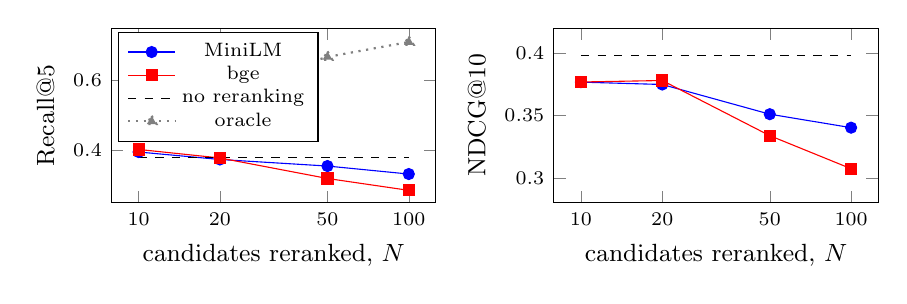
\begin{tikzpicture}
\begin{axis}[name=left, width=0.47\linewidth, height=3.8cm, xmode=log,
  xtick={10,20,50,100}, xticklabels={10,20,50,100}, xlabel={candidates reranked, $N$},
  ylabel={Recall@5}, ymin=0.25, ymax=0.75,
  legend style={font=\scriptsize, at={(0.02,0.98)}, anchor=north west, row sep=-2pt},
  tick label style={font=\scriptsize}, label style={font=\small}]
\addplot[mark=*, blue] coordinates {(10,0.3957) (20,0.3743) (50,0.3555) (100,0.3326)};
\addplot[mark=square*, red] coordinates {(10,0.4030) (20,0.3786) (50,0.3199) (100,0.2859)};
\addplot[dashed, black, domain=10:100] {0.3795};
\addplot[dotted, thick, gray, mark=triangle*] coordinates {(10,0.4740) (20,0.5760) (50,0.6678) (100,0.7106)};
\legend{MiniLM, bge, no reranking, oracle}
\end{axis}
\begin{axis}[at={(left.east)}, anchor=west, xshift=1.5cm, width=0.47\linewidth, height=3.8cm, xmode=log,
  xtick={10,20,50,100}, xticklabels={10,20,50,100}, xlabel={candidates reranked, $N$},
  ylabel={NDCG@10}, ymin=0.28, ymax=0.42,
  tick label style={font=\scriptsize}, label style={font=\small}]
\addplot[mark=*, blue] coordinates {(10,0.3768) (20,0.3749) (50,0.3511) (100,0.3403)};
\addplot[mark=square*, red] coordinates {(10,0.3769) (20,0.3781) (50,0.3339) (100,0.3074)};
\addplot[dashed, black, domain=10:100] {0.3983};
\end{axis}
\end{tikzpicture}
\caption{Retrieval quality on dev (125 questions, means, 0--1) when the top $N$ \texttt{enc\_a} candidates are reranked and the top 5 kept. Dashed: baseline. Dotted: oracle Recall@5, the best any reordering of the top $N$ could reach.}
\label{fig:quality}
\end{figure}

The oracle line in Figure~\ref{fig:quality} rises from 0.47 to 0.71, so a perfect reranker would gain a lot from deeper candidates. Both real rerankers do the opposite: Recall@5 and NDCG@10 fall as $N$ grows, and the larger bge model falls fastest (Recall@5 0.40 at $N{=}10$, 0.29 at $N{=}100$). At $N{=}10$ both are slightly above the baseline on Recall@5 (+1.6 and +2.4 points), but they are below it on NDCG@10 and MRR@10 at every $N$. On practice even $N{=}10$ is below the baseline on Recall@5 (Appendix~\ref{app:rag}), so the small dev gain does not hold across splits.

\label{sec:cost}

\begin{table}[t]
\caption{Reranking cost on dev (benchmark, no ELM calls): ms per question, median (95th percentile) over 5 repeats $\times$ 125 questions after warm-up. Load time varies with disk caching.}
\label{tab:cost}
\centering\small
\setlength{\tabcolsep}{4pt}
\begin{tabular}{lrrrrrr}
\toprule
Model & $N{=}10$ & $N{=}20$ & $N{=}50$ & $N{=}100$ & Peak GPU memory & Load time \\
\midrule
MiniLM (22M) & 32 (36) & 61 (67) & 113 (126) & 169 (194) & 359\,MB & 0.5--2.1\,s \\
bge (278M) & 111 (117) & 220 (228) & 402 (437) & 647 (742) & 1599\,MB & 3.9--31\,s \\
\bottomrule
\end{tabular}
\end{table}

Latency grows roughly in proportion to $N$, one forward pass per candidate, and bge is 3.5--3.8$\times$ slower than MiniLM (Table~\ref{tab:cost}). Inside the answer runs it took longer (96 vs 61\,ms for MiniLM $N{=}20$, 140 vs 111\,ms for bge $N{=}10$), probably because the encoder and reranker share the CPU. For scale, the practice baseline takes a median 9.2\,s per question with ASR (ASR 4.3\,s, embedding 0.18\,s, search 5\,ms, generation 4.2\,s). Our two tested configurations add about 1\%, and bge at $N{=}100$ would add 7\%. GPU memory is the tighter limit: our ASR model peaks at 8.56\,GiB on this 11\,GB card, leaving little room for bge's 1.6\,GB.

\subsection{Reranking: answer quality}
\label{sec:answers}

\begin{table}[t]
\caption{End-to-end results on dev (125 questions, same transcripts, $k{=}5$). Retrieval metrics from the sweep (same deterministic reranking). Judge: mean normalised score (0--1); $\Delta$: mean paired difference from the baseline, 95\% bootstrap CI, sign-flip $p$. Zero: answers scored 0. Rerank and end-to-end (no ASR): medians in ms. Prompt: mean characters.}
\label{tab:main}
\centering\small
\setlength{\tabcolsep}{3.5pt}
\resizebox{\linewidth}{!}{%
\begin{tabular}{lcccccccrr}
\toprule
Configuration & Recall@5 & MRR@10 & NDCG@10 & Judge & $\Delta$ judge [95\% CI], $p$ & Zero & Rerank & Prompt & End-to-end \\
\midrule
Baseline & 0.380 & 0.460 & 0.398 & 0.314 & -- & 56 & -- & 4980 & 5050 \\
MiniLM, $N{=}20$ & 0.374 & 0.428 & 0.375 & 0.305 & $-0.009$ [$-0.065$, $+0.048$], 0.78 & 59 & 96 & 6004 & 5116 \\
bge, $N{=}10$ & 0.403 & 0.419 & 0.377 & 0.349 & $+0.035$ [$-0.021$, $+0.089$], 0.24 & 52 & 140 & 5362 & 4779 \\
\bottomrule
\end{tabular}}
\end{table}

Both confidence intervals in Table~\ref{tab:main} include zero, so we cannot say that either reranker changes answer quality. bge at $N{=}10$ is ahead on all three judge parts (correctness 1.44 vs 1.32, grounding 1.52 vs 1.35, completeness 1.22 vs 1.10, out of 4), but none of these differences is clear either. The end-to-end differences come from the ELM service, not from reranking: the bge run was the fastest despite its longer prompts.

Single judge scores are noisy. Before the main runs we generated answers for 5 practice questions twice, with identical transcripts and identical top-5 records. The answers differed every time (temperature 0.1), and with the same judge model and rubric 4 of the 5 scores changed: the mean absolute change was 0.15, and one score moved by 0.5. On dev, for the 5 questions where a reranker picked the same 5 records as the baseline, 3 still got a different score. So we compare means over all 125 paired questions, not counts of wins (bge: 35 better, 26 worse; MiniLM: 32 and 30).

\subsection{Why reranking does not help here}
\label{sec:why}

Better evidence does give better answers. In the dev baseline, the 52 questions with no relevant record in the top 5 have a mean judge score of 0.12, against 0.45 for the other 73 (practice: 0.14 for 143 questions, 0.47 for 207), and 37 of the 56 zero-score answers have Recall@5${}=0$. The reranked runs agree. With bge, the 17 questions whose Recall@5 rose gained 0.18 on average (8 better, 1 worse) and the 11 whose Recall@5 fell lost 0.05; with MiniLM, the 19 that gained Recall@5 rose by 0.10 and the 17 that lost it fell by 0.17.

The problem is that the rerankers rarely improve the evidence. They raised Recall@5 for only 17--19 dev questions and lowered it for 11--17, and they moved correct first results down. The baseline has a relevant record at rank 1 for 47 dev questions; MiniLM $N{=}20$ keeps 33 of them and bge $N{=}10$ keeps 28. The 8 and 10 new rank-1 hits do not make up for this, so MRR@10 falls in every configuration.

The most likely cause is a domain mismatch: MiniLM was trained on web-search queries and bge on general data, while our records are long, informal forum posts and our questions come through ASR. Cross-encoders often lose much of their advantage on new domains~\citep{thakur2021beir}, and two results fit this. Quality falls as $N$ grows: deeper candidates are mostly off-topic, and each one is another chance for a plausible but irrelevant post to win. And the larger bge model does worse than the small one at large $N$, so more capacity does not fix it.

We checked four other explanations. \emph{Longer prompts:} the rerankers prefer longer records, so prompts grew by 21\% (MiniLM) and 8\% (bge), but the change in prompt length hardly predicts the change in judge score (correlation 0.03 and 0.15), and among questions whose Recall@5 did not change, longer and shorter prompts differ by at most 0.03 in mean score. Prompt length is a cost here, not the cause. \emph{Truncation:} 9.7\% and 11.5\% of pairs exceed 512 tokens and lose their end; this is too rare to explain why 30--40\% of the correct first results moved down, though we did not test it directly. \emph{ASR errors:} all conditions share the transcripts, so ASR errors cannot explain differences between them. \emph{Judge noise:} it widens the intervals in Table~\ref{tab:main} but cannot explain the retrieval metrics.

\section{Discussion and conclusion}
\label{sec:conclusion}

Our ASR kernels are correct and the memory-bound ones are fast (RoPE reaches 80\% of peak bandwidth), but the simple tiled GEMM, 83\% of the time and 7--10$\times$ below cuBLAS, makes the model 3.0$\times$ slower than PyTorch. Register tiling in GEMM, and a KV cache in the decoder, are the next steps.

For RAG, our evidence supports a narrow conclusion. On this corpus, an off-the-shelf cross-encoder after \texttt{enc\_a} costs 32--647\,ms per question, up to 1.6\,GB of GPU memory and up to 21\% longer prompts, and gives no measurable gain in answer quality. Answers do improve when Recall@5 improves, so the idea behind reranking holds; these two rerankers just do not rank this corpus better than the supplied encoder. A reranker fine-tuned on in-domain question--record pairs, or a combined score that only lets the reranker reorder records \texttt{enc\_a} already ranks highly, might change this; we did not test either.

\textbf{Limitations.} With 125 dev questions the 95\% interval of the mean judge difference is about $\pm0.055$, so smaller effects would go unseen. Each answer was judged once, by the model that wrote it, from the ASR transcript rather than the original question. All timings come from one GPU type and a shared ELM service, and $N$ was chosen on practice, not on dev.


% References are excluded from the main-body page limit.
\bibliography{references}
\bibliographystyle{iclr2027_conference}

\appendix
\section{HW1 outputs}
\label{app:hw1}
These are the saved outputs of \texttt{nvidia-smi -L} and \texttt{make test}, followed by both profiles in Table~\ref{tab:profile-full}, all from one session on one node. Compiler command lines and the library path are left out.

{\tiny
\begin{verbatim}
$ nvidia-smi -L
GPU 0: NVIDIA GeForce RTX 2080 Ti

$ make test     (each test first prints the GPU: RTX 2080 Ti, sm_75, 68 SMs, peak bandwidth about 616 GB/s)
tiny (2 x 3 tokens, Hq=3, Hk=1)      PASS  max_err=1.08e-07     0.004 ms      0.4 GB/s ( 0% of peak)
odd sizes, partial rotation          PASS  max_err=1.08e-07     0.004 ms      4.0 GB/s ( 1% of peak)
audio encoder (partial, 32/64)       PASS  max_err=1.93e-07     0.031 ms    490.1 GB/s (80% of peak)
text decoder (GQA 16/4, full)        PASS  max_err=1.64e-07     0.004 ms    297.0 GB/s (48% of peak)
Task 1 (RoPE): ALL PASS
rmsnorm, one short row               PASS  max_err=8.27e-08     0.004 ms      0.1 GB/s ( 0% of peak)
rmsnorm, odd cols                    PASS  max_err=3.68e-07     0.004 ms      9.7 GB/s ( 2% of peak)
rmsnorm, text decoder                PASS  max_err=4.35e-07     0.006 ms    164.6 GB/s (27% of peak)
layernorm, odd cols (example)        PASS  max_err=3.91e-07     0.005 ms      8.3 GB/s ( 1% of peak)
layernorm, audio encoder             PASS  max_err=5.42e-07     0.040 ms    381.7 GB/s (62% of peak)
softmax, one short row               PASS  max_err=1.11e-08     0.005 ms      0.0 GB/s ( 0% of peak)
softmax, odd cols                    PASS  max_err=1.04e-09     0.004 ms      5.5 GB/s ( 1% of peak)
softmax, large inputs (+-100)        PASS  max_err=2.67e-08     0.005 ms      3.2 GB/s ( 1% of peak)
softmax, all negative (-200..-150)   PASS  max_err=6.11e-09     0.004 ms      1.2 GB/s ( 0% of peak)
softmax, vocabulary row (59264)      PASS  max_err=8.13e-11     0.131 ms      3.6 GB/s ( 1% of peak)
softmax, 64 x 4096                   PASS  max_err=7.95e-10     0.010 ms    220.3 GB/s (36% of peak)
Task 2 (reductions): ALL PASS
tiny 3 x 5, K = 7                    PASS  max_err=9.76e-09     0.004 ms        0 GFLOP/s
    for comparison: naive      0 GFLOP/s, cuBLAS      0 GFLOP/s (CPU reference)
odd sizes 37 x 100, K = 33, bias     PASS  max_err=1.55e-07     0.004 ms       60 GFLOP/s
    for comparison: naive     50 GFLOP/s, cuBLAS     22 GFLOP/s (CPU reference)
odd sizes, bias + GELU               PASS  max_err=7.70e-07     0.007 ms      126 GFLOP/s
    for comparison: naive     86 GFLOP/s, cuBLAS     87 GFLOP/s (CPU reference)
decoder q_proj (64x2048x2048)        PASS  max_err=1.10e-05     0.439 ms     1224 GFLOP/s
    for comparison: naive    153 GFLOP/s, cuBLAS   4656 GFLOP/s (cuBLAS reference)
decoder gate_proj (64x6144x2048)     PASS  max_err=1.19e-05     1.218 ms     1322 GFLOP/s
    for comparison: naive    161 GFLOP/s, cuBLAS   6823 GFLOP/s (cuBLAS reference)
decoder down_proj (64x2048x6144)     PASS  max_err=3.62e-05     1.234 ms     1306 GFLOP/s
    for comparison: naive    185 GFLOP/s, cuBLAS   8058 GFLOP/s (cuBLAS reference)
lm_head, last token (1x59264x2048)   PASS  max_err=1.24e-05     1.945 ms      125 GFLOP/s
    for comparison: naive    117 GFLOP/s, cuBLAS    291 GFLOP/s (cuBLAS reference)
encoder q_proj (1500x1280x1280)      PASS  max_err=2.38e-07     2.534 ms     1939 GFLOP/s
    for comparison: naive    234 GFLOP/s, cuBLAS  13195 GFLOP/s (cuBLAS reference)
encoder fc1 + GELU (1500x5120x1280)  PASS  max_err=6.92e-07    14.205 ms     1384 GFLOP/s
    for comparison: naive    235 GFLOP/s, cuBLAS  13384 GFLOP/s (cuBLAS reference)
conv2 via im2col (1500x1280x3840)    PASS  max_err=7.16e-07    10.113 ms     1458 GFLOP/s
    for comparison: naive    234 GFLOP/s, cuBLAS  13705 GFLOP/s (cuBLAS reference)
Task 3 (tiled GEMM): ALL PASS
tiny, one tile (4 queries, 5 keys)   PASS  max_err=1.11e-07     0.005 ms        1 GFLOP/s
several tiles, peaky scores          PASS  max_err=4.97e-07     0.013 ms       17 GFLOP/s
GQA 4 heads / 2 kv heads             PASS  max_err=1.30e-07     0.006 ms       93 GFLOP/s
causal, seq_q = seq_k                PASS  max_err=4.86e-07     0.025 ms      100 GFLOP/s
causal, 5 new queries, 37 keys       PASS  max_err=1.78e-07     0.007 ms       26 GFLOP/s
causal, one new query                PASS  max_err=3.39e-07     0.023 ms       25 GFLOP/s
text decoder (GQA 16/4, causal)      PASS  max_err=5.21e-07     0.063 ms      266 GFLOP/s
audio encoder (20 heads, 1500)       PASS  max_err=2.68e-07    11.136 ms     1034 GFLOP/s
Task 4 (attention): ALL PASS
\end{verbatim}
}

\begin{table}[h]
\caption{Output of \texttt{./run.sh --profile} (ours: all tasks on our kernels) and \texttt{./run.sh --cuda none --profile} (PyTorch), copied from the saved files into one table. Both runs used the 3.5\,s test clip (mel features $1\times128\times3000$, a prompt of 59 tokens) and both produced the transcription ``Concord returned to its place amidst the tents.''}
\label{tab:profile-full}
\centering\small
\setlength{\tabcolsep}{4pt}
\begin{tabular}{lrrrrrr}
\toprule
 & \multicolumn{3}{c}{Ours} & \multicolumn{3}{c}{PyTorch} \\
\midrule
Model load time (s), not in the timings & \multicolumn{3}{r}{72.6} & \multicolumn{3}{r}{29.3} \\
Timed runs, 13 tokens each (ms) & \multicolumn{3}{r}{3222.1 / 3230.1 / 3239.6} & \multicolumn{3}{r}{1065.3 / 1065.0 / 1064.7} \\
Time per transcription, mean $\pm$ std (ms) & \multicolumn{3}{r}{$3230.6 \pm 7.2$} & \multicolumn{3}{r}{$1065.0 \pm 0.2$} \\
Time per token (ms) & \multicolumn{3}{r}{248.5} & \multicolumn{3}{r}{81.9} \\
Peak GPU memory (GiB) & \multicolumn{3}{r}{8.56} & \multicolumn{3}{r}{8.88} \\
Word accuracy, status & \multicolumn{3}{r}{100.0\%, PASS} & \multicolumn{3}{r}{100.0\%, PASS} \\
\midrule
Operation (profiled transcription) & calls & ms & share & calls & ms & share \\
\midrule
\texttt{linear} & 2757 & 2832.1 & 83.3\% & 2757 & 597.4 & 41.6\% \\
\texttt{attention} & 396 & 547.3 & 16.1\% & 396 & 313.3 & 21.8\% \\
\texttt{rmsnorm} & 741 & 6.7 & 0.2\% & 741 & 85.5 & 5.9\% \\
\texttt{rope} & 396 & 3.0 & 0.1\% & 396 & 433.3 & 30.1\% \\
\texttt{silu\_mul} & 364 & 3.6 & 0.1\% & 364 & 4.0 & 0.3\% \\
\texttt{layernorm} & 65 & 2.4 & 0.1\% & 65 & 2.6 & 0.2\% \\
\texttt{softmax} & 13 & 1.6 & 0.0\% & 13 & 0.3 & 0.0\% \\
\texttt{embedding} & 13 & 1.5 & 0.0\% & 13 & 1.0 & 0.1\% \\
\texttt{im2col} & 2 & 0.2 & 0.0\% & 2 & 0.3 & 0.0\% \\
Total GPU time in kernels & & 3398.5 & & & 1437.7 & \\
\bottomrule
\end{tabular}
\end{table}

\section{Reranking: full results}
\label{app:rag}

\begin{table}[h]
\caption{Retrieval sweep on both splits: Recall@5 / NDCG@10 / MRR@10, and the median rerank time on dev (ms). Recall@100 is the same in every row by construction (practice 0.770, dev 0.724), which we used as a check of the metric code.}
\centering\small
\resizebox{\linewidth}{!}{%
\begin{tabular}{lccr}
\toprule
Configuration & Practice (350 questions) & Dev (125 questions) & Rerank ms (dev) \\
\midrule
Baseline (no reranking) & 0.421 / 0.420 / 0.489 & 0.380 / 0.398 / 0.460 & -- \\
MiniLM, $N{=}10$ & 0.404 / 0.405 / 0.464 & 0.396 / 0.377 / 0.424 & 32 \\
MiniLM, $N{=}20$ & 0.411 / 0.414 / 0.471 & 0.374 / 0.375 / 0.428 & 61 \\
MiniLM, $N{=}50$ & 0.399 / 0.399 / 0.454 & 0.356 / 0.351 / 0.412 & 112 \\
MiniLM, $N{=}100$ & 0.388 / 0.395 / 0.453 & 0.333 / 0.340 / 0.400 & 167 \\
bge, $N{=}10$ & 0.392 / 0.382 / 0.428 & 0.403 / 0.377 / 0.419 & 108 \\
bge, $N{=}20$ & 0.377 / 0.371 / 0.408 & 0.379 / 0.378 / 0.426 & 215 \\
bge, $N{=}50$ & 0.351 / 0.340 / 0.383 & 0.320 / 0.334 / 0.396 & 398 \\
bge, $N{=}100$ & 0.327 / 0.313 / 0.353 & 0.286 / 0.307 / 0.359 & 643 \\
\midrule
Oracle Recall@5, $N = 10/20/50/100$ & 0.477 / 0.575 / 0.679 / 0.764 & 0.474 / 0.576 / 0.668 / 0.711 & \\
\bottomrule
\end{tabular}}
\end{table}

On practice we chose MiniLM at $N{=}20$ and bge at $N{=}10$, the setting with the highest Recall@5 for each model. The practice baseline answers scored 0.335 on average (350 questions; 135 scored 0). In the latency benchmark, throughput rises with $N$ (MiniLM 342 to 593 pairs/s, bge 99 to 155 pairs/s), because larger $N$ fills the batches of 32 better.

% Keep this line unchanged.
\newpage

% Academic integrity is an underlying principle of research and academic practice.
% All submitted work is expected to be your own, including any material you have
% generated yourself with the assistance of AI tools such as ELM, ChatGPT,
% Bing Chat, Claude, Google Gemini, or any other automated assistance.
% For all such material you must make prominent explicit acknowledgement and
% explain clearly what you have done in this section.
% This includes using AI to directly generate text, code, figures or similar
% or to complete other tasks. In all cases, you remain entirely responsible
% for the material you produce.
\section*{AI declaration}
{\raggedright
We used Claude Code (Anthropic) during this coursework, as follows.
\begin{itemize}
\item HW1: it explained CUDA ideas (warp shuffles, tiling, online softmax), helped us debug our kernels, checked the numbers in our answers to the task-guide questions and helped reword those answers.
\item RAG investigation: it wrote the fallback parser for malformed judge output and, from a plan we agreed with it, the reranking code: \texttt{rag/extensions/reranker.py}, \texttt{rag/extensions/bench\_rerank.py}, \texttt{rag/scripts/evaluate\_rerank.py}, the changes to \texttt{rag/src/rag.py} and \texttt{rag/scripts/generate\_answers.py}, and \texttt{rag/tests/test\_rerank.py}. It also proposed the experiment design, gave us the cluster commands and wrote the scripts for the paired analysis.
\item Report: it drafted the text, tables and figures of this report from our result files. We checked the numbers against those files and edited the text.
\end{itemize}
We ran every experiment on the cluster ourselves and take full responsibility for all of the content. The University ELM service (EuroLLM-22B-Instruct) is part of the system itself, as the answer generator and the judge.\par}

% Please put the information of your group here without changing the format.
% This page will be deleted when the report is distributed for reviewing.
\section*{Group information}
Group ID: XXX

Information of group member A:
\begin{itemize}
    \item Name: John Doe
    \item UUN: sXXXXXXX
\end{itemize}

% Second member (the group has two members).
Information of group member B:
\begin{itemize}
    \item Name: John Doe
    \item UUN: sXXXXXXX
\end{itemize}

% Keep this COMMENTED OUT, unless there is more than one member and you feel like
% it is necessary to point out the contribution. Please notice that members from
% the same group technically receive the same score for the report, regardless of
% the contribution.
% \section*{Contribution}

\end{document}
